\unnumberedChapter[analysisArchitecturalApproaches]{Analysis of Architectural Approaches}

\unnumberedSection[modifiability]{Modifiability}

\ATAM{M1}{Add different game levels/designs}
{Modifiability}
{Wish to add different level designs}
{Make changes, unit testing, possibly user testing. In 3 hours, levels will be integrated in the system without
adapting other modules}
{\textbf{Observer} & \nameref{s4} & & \nameref{r3}, \nameref{r4} & \\
\textbf{Template Method} & & \nameref{t2} & \nameref{r5} & \\}
{\begin{itemize}
  \item Observer pattern will be used to notify the other bricks constituting the castle after the destruction of a brick for the repercussion on the remaining structure.
  \item Template Method pattern could be used to define the generic initialisation of the world by varying the procedures to be used to incorporate new game elements or induce more randomness per example.
\end{itemize}}
{\newline
\begin{minipage}{0.5\textwidth}
  \centering
  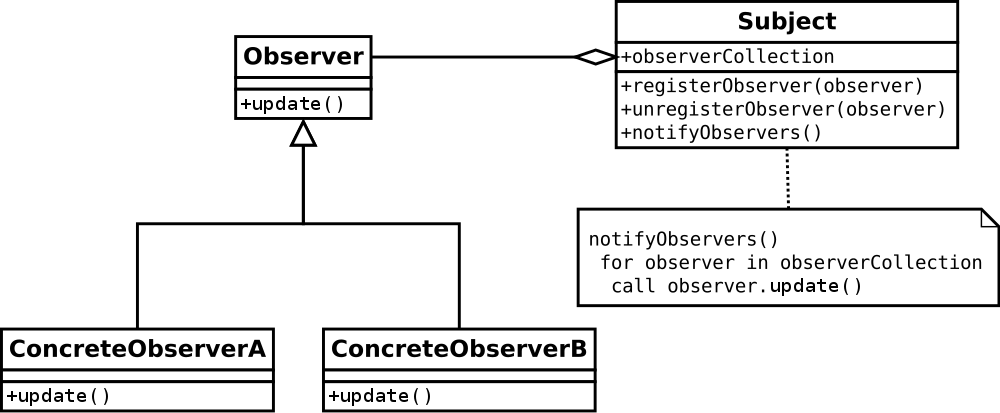
\includegraphics[width=\textwidth,height=0.4\textheight,keepaspectratio]{observerPatternClassDiagram}
\end{minipage}
\hfill
\begin{minipage}{0.3\textwidth}
  \centering
  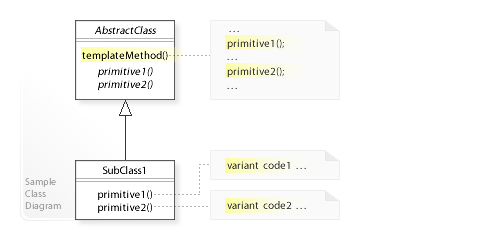
\includegraphics[width=\textwidth,height=0.3\textheight,keepaspectratio]{templateMethodPatternClassDiagram}
\end{minipage}
\vspace{1mm}}


\unnumberedSection[availability]{Availability}
Availability will be about detecting and preventing faults, as well as be able to recover from them.

\ATAM{A1}{Detecting and recovering from player losing connection}
{Availability}
{Normal operations}
{One player looses connection. Return to main menu with an error message that the opponent is disconnected.}
{\textbf{Ping/Echo} & \nameref{s1} & & \nameref{r1} & \\
\textbf{\gls{p2p} Connection} & \nameref{s2}, \nameref{s3} & & & \nameref{n1} \\}
{\begin{itemize}
  \item Ping/Echo ensure that the game participants will know when a user is no longer connected to the game.
  \item \gls{p2p} will ensure that the only connected players can do the ping directly at participants, reducing the need for a server to notify it for you.
\end{itemize}}
{\begin{center}
  \vspace{0em}
  \hspace{5em}
  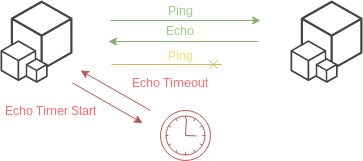
\includegraphics[width=0.5\textwidth,height=0.3\textheight,keepaspectratio]{pingEchoATAM}
\end{center}}

\ATAM{A2}{Detecting players' game state out of sync and recovery}
{Availability}
{Normal operations}
{One player's game state update is not notified to other participants. Use game state that was last accepted by both devices.}
{\textbf{\gls{p2p} Connection} & \nameref{s2}, \nameref{s3} & & & \nameref{n1} \\
\textbf{State \newline Resynchronisation} & & \nameref{t1} & \nameref{r2} & \\}
{\begin{itemize}
  \item \gls{p2p} connection will create a channel for where the clients can share their latest accepted game state
  \item State resynchronisation will assure the clients that the state they are using, is the latest agreed game state, so that nobody will play on a different game state than their opponent
\end{itemize}}
{\begin{center}
  \vspace{-1em}
  \hspace{5em}
  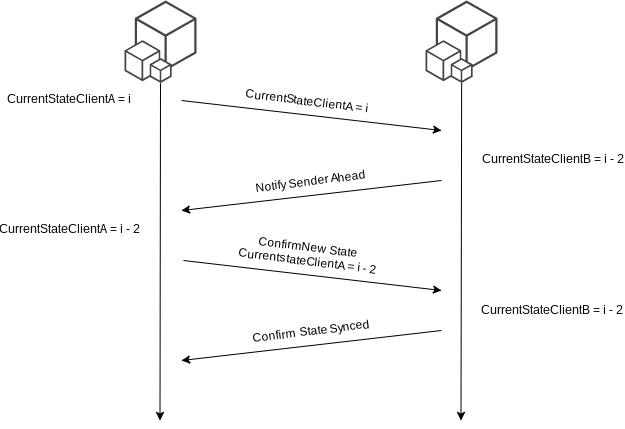
\includegraphics[width=\textwidth,height=0.4\textheight,keepaspectratio]{p2pATAM}
\end{center}}

% DO NOT REMOVE WEIRD END OF FILE ERROR SPAWNING...
